\setcounter{figure}{0}
\renewcommand{\thefigure}{S\arabic{figure}}
\providecommand{\theHfigure}{\thefigure}
\renewcommand{\theHfigure}{SI.\arabic{figure}}
\setcounter{table}{0}
\renewcommand{\thetable}{S\arabic{table}}
\providecommand{\theHtable}{\thetable}
\renewcommand{\theHtable}{SI.\arabic{table}}

\begin{figure}[htbp]
    \centering
    \includegraphics[width=\linewidth]{figures/low_lying_state_errors/error_distribution_6e6o.png}
    \caption{UCCSD low-lying-state error distribution in the $6e6o$ active space.}
    \label{fig:si-error-distribution}
\end{figure}

\begin{figure}[htbp]
    \centering
    
\includegraphics[width=\linewidth]{figures/spin_contamination/bad_spin_roots_6e6o.png}
    \caption{Spin-contaminated roots across ansatz families in the $6e6o$ active space.}
    \label{fig:si-spin-contaminated-roots}
\end{figure}

\input{tables/results/table_S1_spin_contamination}

\input{tables/results/table_s2_spin_mean_trotter}

\begin{figure}[htbp]
    \centering
    
\includegraphics[width=\linewidth]{figures/overlap_eigenvalue_spread/1upccgsdsinglet_triplet_6e6o.png}
    \caption{1UpCCGSDSinglet overlap-eigenvalue spread for the $6e6o$ singlet and triplet sectors.}
    \label{fig:si-1up-triplet-eigenvalues}
\end{figure}

\begin{figure}[htbp]
    \centering
    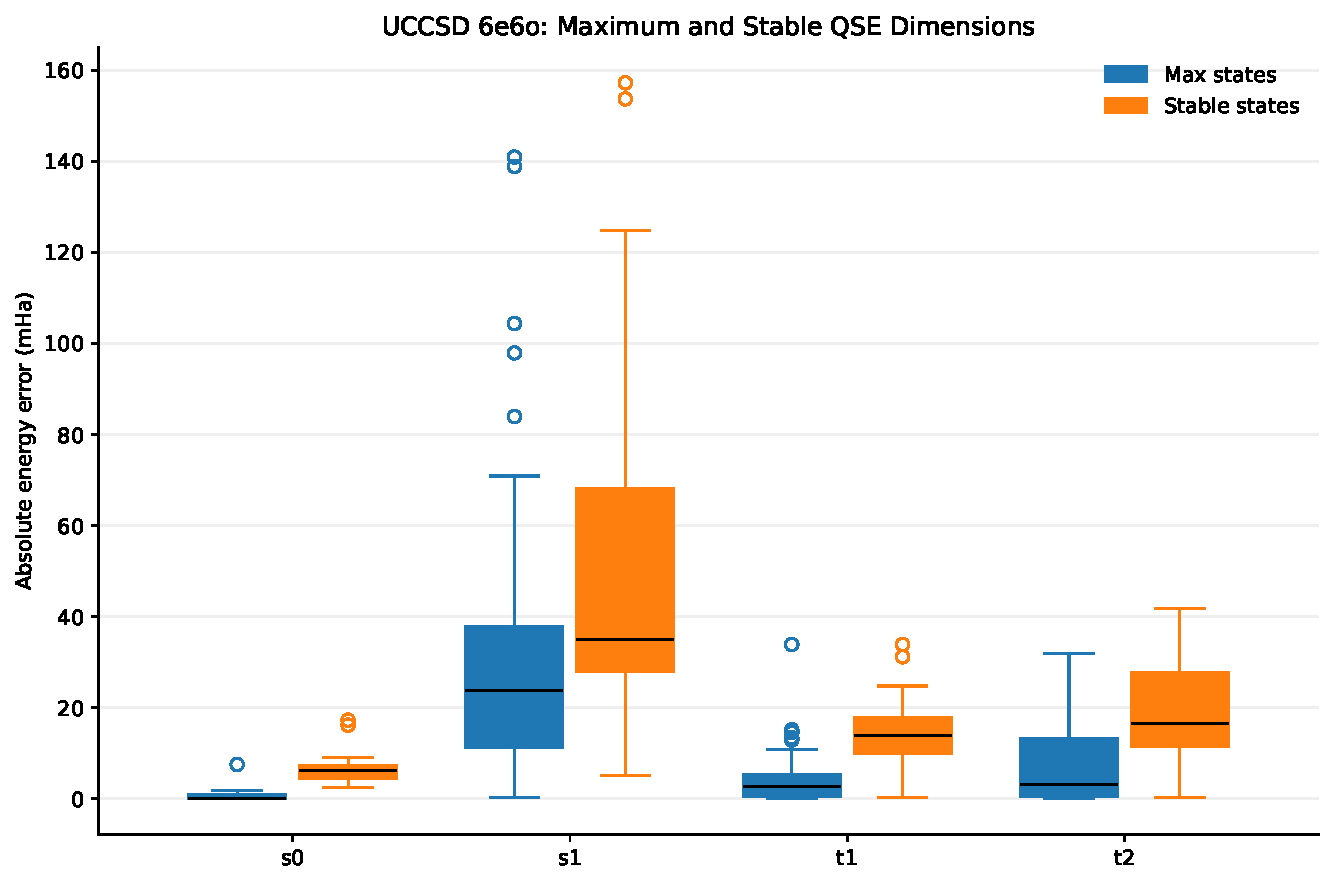
\includegraphics[width=\linewidth]{figures/dimension_analysis/max_stable_error_distribution_6e6o.png}
    \caption{Molecule-level index-matched errors for the low-lying $s0$, $s1$, $t1$, and $t2$ roots in the UCCSD $6e6o$ active space, comparing the maximum retained QSE dimension with the overlap-stable dimension.}
    \label{fig:si-max-stable-error-distribution}
\end{figure}

\begin{figure}[htbp]
    \centering
    
\includegraphics[width=\linewidth]{figures/shots/eigenvalue_lifting/uccsd_6e6o.png}
    \caption{Finite-shot lifting of UCCSD overlap eigenvalues in the $6e6o$ active space.}
    \label{fig:si-eigenvalue-lifting}
\end{figure}

\begin{figure}[htbp]
    \centering
    
\includegraphics[width=\linewidth]{figures/matrix_heatmaps/uccsd_6e6o_singlet_overlap.png}
    \caption{Full 28-molecule singlet overlap heatmaps comparing statevector and shot-based results.}
    \label{fig:si-full-singlet-heatmaps}
\end{figure}

\begin{figure}[htbp]
    \centering
    
\includegraphics[width=\linewidth]{figures/matrix_heatmaps/uccsd_6e6o_triplet_overlap.png}
    \caption{Full 28-molecule triplet overlap heatmaps comparing statevector and shot-based results.}
    \label{fig:si-full-triplet-heatmaps}
\end{figure}
